\documentclass[12pt]{paper}

\usepackage{microtype,tikz,mathptmx,helvet,enumitem,listings} 
\usepackage[margin = 1in]{geometry}

\setlist[enumerate]{leftmargin=*}
\lstset{basicstyle=\ttfamily,language=TeX,keywordstyle=\ttfamily}

\title{Tips and Tricks}
\author{Math 351}
\date{}

\begin{document}

\maketitle

This final week of Math 351 is for final design tips and for introducing some useful packages and
commands we haven't yet encountered.  Thank you for your hard work this quarter, I hope
you've gotten something out of our course.

\section{Design tips}

\begin{enumerate}

\item Read the package or class documentation!  The answers to typesetting
  questions are in the documentation.

  Our textbook and the example \verb~.tex~ files from Math 351 are other places to find quality
  typesetting advice.  Warning: sometimes the answers on random websites and message board site
  such as stackexchange can be outdated and incorrect.

\item Do not copy or paste long, mysterious preambles from other \verb~.tex~ documents without
  understanding the commands (this goes along with reading the documentation).

\item Before defining an newcommand or environment, check CTAN to see if someone has already
  done the work.  For example, don't come up with your own way to denote modular operations; for
  that there is the predefined commands \verb~\pmod~ and \verb~\bmod~ which can be used in this
  way: $a = b \pmod c$ and $a\bmod c = b$
  
\item Write the document first and make visual formatting choices later.  Focus on content and do not
  fiddle with formatting too much while writing.

\item Spacing commands such as \verb~\\~, \verb~\vspace~, \verb~\newpage~, or \verb~\par~ are
  rarely needed.
  
\item Graphics need to be of high quality.  Never use pixelated or low resolution images.  
  
\item If there is a long unbreakable word (see the \verb~\mbox~ command) or a long
  mathematics equation, \LaTeX{} might place part of the long expression in the margins.
  If this happens, the compiler will register an ``\verb~Overfull \hbox~'' error.
  Avoid this, usually by using \verb~\gather~, \verb~\multiline~, or \verb~\align~ for
  long mathematical equations.

\item Use \verb~\emph~ to \emph{emphasize} text instead of using \verb~\textbf~ or underlining.

\end{enumerate}

\section{Tricks and sometimes useful commands}

\begin{enumerate}

\item The \verb~minipage~ environment creates a smaller page within a page,
  useful for side by side type:
\begin{center}
\begin{minipage}{15eM}
This is left text.
\end{minipage}
\begin{minipage}{15eM}
\begin{lstlisting}
\begin{minipage}{15eM}
This is left text.
\end{minipage}
\begin{minipage}{15eM}
This is right text.
\end{minipage}
\end{lstlisting}
\end{minipage}
\end{center}

\item The \verb~figure~ and \verb~table~ environments create floating figures or
tables (floating means \LaTeX{} decides the best placement of the figure).  The options 
\verb~h~, \verb~t~, or \verb~b~ tell \LaTeX{} to attempt placing the figure here, top, or bottom
of the page, respectively.  To have words wrap around the figures, use the \verb~wrapfig~ package.
\begin{figure}[h]
\begin{center}
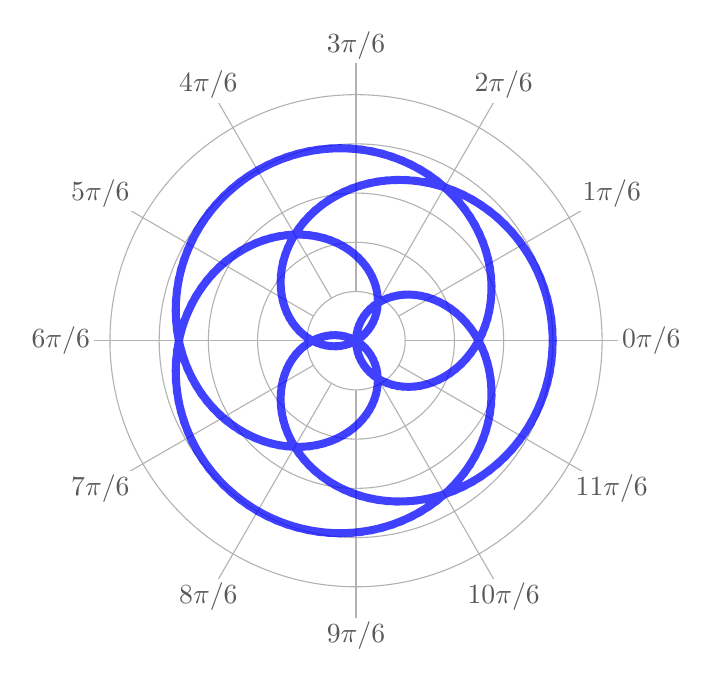
\begin{tikzpicture}[scale = 2.5]
\foreach \x in {0,...,11} \draw [black!30] (\x*30:.25) -- (\x*30:1.5) node [black!66, fill = white, inner sep = .5mm] {$\x \pi/6$};
\foreach \x in {1,...,5} \draw [black!30] (0,0) circle (\x/4); 
\draw [domain = 0:360*7, blue, samples = 400, line width = 1mm, opacity=.75] plot (\x:{cos(3*\x/7)});
\end{tikzpicture}
\end{center}
\caption{The polar equation $r = \cos(3 x/7)$ provides an example of a floating figure.}
\end{figure}

\item The compiler makes typesetting decisions by placing boxes around letters, parts of 
words, mathematics, and figures, and then appropriately arranging the boxes.  Force unbreakable type
to reside in a single box using \verb~\mbox{unbreakable text}~.  Create a frame around a box 
using \verb~\fbox{.}~ and an unbreakable paragraph using \verb~\parbox{width}{.}~.  

Sometimes when using commands such as \verb~\hfill~, an empty box is needed to get
spacing just right; create such an empty box with \verb~\mbox{}~.

On a similar note, \verb!~! is a non-breaking space character, used when a space between two 
words or characters should appear but those words cannot be on different lines.

\item Separate multiple authors using \verb~\and~ within the \verb~\author~ command.

\item Double spacing is achieved by placing \verb~\linespread{1.6}~ in the preamble.

\item Most of us are familiar with tabs from our frequent use of physical typewriters. 
Tabs can be kept and used with the \verb~tabbing~ environment.  Set tabs using \verb~\=~, 
create a new line using \verb~\\~, and move to the next tab using \verb~\>~.  For example,
\begin{tabbing}
The first tab appears right here, \= this is text after the first tab, \= and there is a third tab.
\\
This is the second row, \>  middle of second row, \> and the end.
\end{tabbing}
is created using
\begin{lstlisting}
\begin{tabbing}
The first tab appears right here, \= 
this is text after the first tab, \= 
and there is a third tab. \\
This is the second row, \>  
middle of second row, \> 
and the end.
\end{tabbing}
\end{lstlisting}
Tabbing environments are treated as one box and thus cannot be split across two pages.

\item Custom counters can be defined using the syntax 
\begin{lstlisting}
\newcounter{countername}
\setcounter{countername}{1}
\end{lstlisting}
in the preamble. The current value of the counter can be accessed using 
\verb~\thecountername~ and incremented using \verb~\addtocounter{countername}{1}~.
Counters work well in tandem with newcommands or newenvironments. 
\end{enumerate}

\end{document}
